\section{Resistenz gegen Overfitting}
% \subsection{Neueste Forschungsergebnisse}
% \subsection{Zukünftige Potenziale von Boosting-Algorithmen}
Overfitting beschreibt das Phänomen, dass durch viele Trainingsiterationen das Modell so gut an die Trainingsdaten angepasst ist, dass es nicht mehr genug generalisiert und mit zunehmenden Iterationen sich der Testfehler erhöht.

\begin{figure}[H]
    \centering
    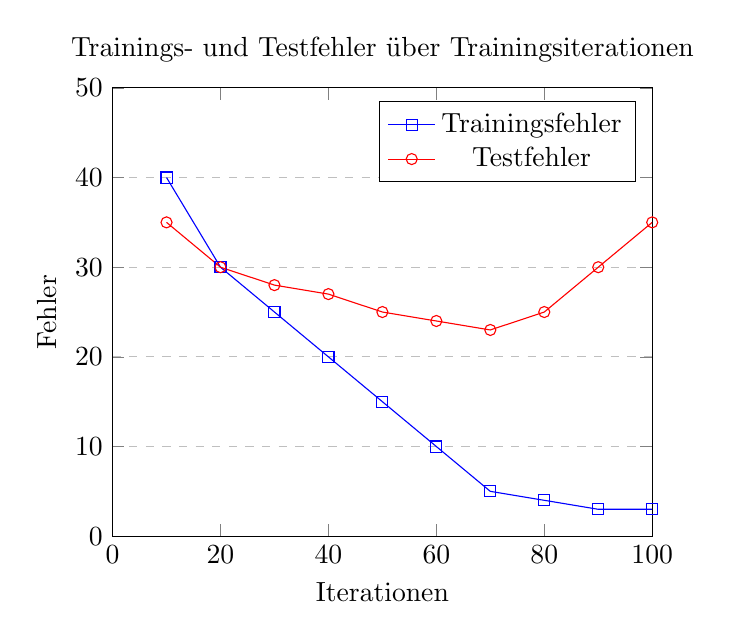
\begin{tikzpicture}
    \begin{axis}[
        title={Trainings- und Testfehler über Trainingsiterationen},
        xlabel={Iterationen},
        ylabel={Fehler},
        xmin=0, xmax=100,
        ymin=0, ymax=50,
        legend pos=north east,
        ymajorgrids=true,
        grid style=dashed,
    ]
    
    \addplot[
        color=blue,
        mark=square,
        ]
        coordinates {
        (10,40)(20,30)(30,25)(40,20)(50,15)(60,10)(70,5)(80,4)(90,3)(100,3)
        };
        \addlegendentry{Trainingsfehler}
    
    \addplot[
        color=red,
        mark=o,
        ]
        coordinates {
        (10,35)(20,30)(30,28)(40,27)(50,25)(60,24)(70,23)(80,25)(90,30)(100,35)
        };
        \addlegendentry{Testfehler}
    
    \end{axis}
    \end{tikzpicture}
    \caption{Hypothetische Darstellung von Overfitting: Während der Trainingsfehler mit zunehmenden Iterationen abnimmt, beginnt der Testfehler nach einem gewissen Punkt wieder zu steigen.}
\end{figure}


\subsection{AdaBoost und die Herausforderung des Overfittings}
In \textcite[Kapitel 1.2.3]{SchapireFreund2012} wird das Phänomen des Overfitting für AdaBoost gezeigt. Trotz dieses theoretischen Hintergrunds war es mir in meinen praktischen Experimenten mit der SKLearn-Bibliothek in Python nicht möglich, Overfitting bei AdaBoost zu reproduzieren. Meine unzähligen Versuche mit unterschiedlichsten Anpassungen führten nicht zu den erwarteten Ergebnissen. Dies führt zu der Frage, warum AdaBoost in meinen Experimenten anscheinend resistent gegen Overfitting war. Der folgende Teil ist meine Theorie zu diesem Phänomen und entspricht nicht zwangsweise dem tatsächlichen Grund.

\subsection{Wahl des Datensatzes} 
Ich habe mich für einen der vielen Varianten an Datensätzen entschieden um Overfitting möglichst zu provozieren:

\begin{lstlisting}
    X, y = make_classification(n_samples=200, n_features=2, n_informative=2, n_redundant=0, n_clusters_per_class=1, flip_y=0.4, random_state=1)
\end{lstlisting}    
Ein relevanter Punkt ist die Menge der Datenpunkte `n\_samples'. Ist dieser zu hoch 
gewählt, ist es für das Modell zu leicht zu generalisieren. Mit den hier gewählten 200 Datenpunkten neigte AdaBoost schon deutlich eher zum Overfitting als beispielsweise mit 10,000.
\newline
Ein zusätzlicher Teil ist die Auswahl Attribute. In dem Datensatz werden zwei Attribute `n\_features' verwendet. Normalerweise würde dies gut klassifizierbare Daten erstellen. Allerdings werden 40\% der Datenwerte hier mittels `y\_flip' umgekehrt. Dies führt zu einem sehr schlecht klassifizierbaren Datensatz.

\subsection{Ergebnisanalyse}
\begin{figure}[h]
    \centering
    \includegraphics[width=0.8\textwidth]{Images/AdaBoost_Error_Plot.png}
    \caption{Trainings- und Testfehler des AdaBoost-Modells über die Iterationen.}
    \label{fig:adaboost_error_plot}
\end{figure}
In \autoref{fig:adaboost_error_plot} sind die Ergebnisse des AdaBoost-Algorithmus dargestellt. Interessanterweise zeigt sich, dass obwohl der Trainingsfehler stetig abnimmt, der Testfehler nicht in dem Maße ansteigt, wie man es bei klassischem Overfitting erwarten würde. Stattdessen bleibt er sehr konstant.

\subsection{Philosophisches Prinzip: Occams Racor}
Occams Racor, oder auf deutsch Occams Rasiermesser ist ein philosophisches Prinzip, welches besagt, dass wenn es zwei Hypothesen zu einer Theorie gibt, dass die simplere vorzuziehen ist. Im Kontext des maschinellen Lernens, bedeutet dies, dass einfacherer Modelle den komplexeren vorzuziehen sind, da es anzunehmen ist, dass sie besser generalisieren. Dieses Prinzip suggeriert, dass bei der Klassifizierung unseres speziellen Datensatzes ein einfacheres Modell mit 250 Iterationen effektiver ist als das Endmodell mit 500 Iterationen, da es weniger anfällig für das "Auswendiglernen" spezifischer Muster der Trainingsdaten und somit für Overfitting ist.

\subsection{Erklärungsansatz: Margins Theorie}
Eine offensichtliche Antwort scheint zu sein, dass die Gewichtung \( \alpha \) des neuen Lerners schnell gegen 0 geht, sobald der Traingsfehler gegen 0 geht. Dies ist vielleicht eine Begründung ab der 250. Iteration, an der der Trainingsfehler 0 erreicht. Die Frage bleibt aber, warum sich bis dahin der Testfehler nicht verschlechtert, da sich das Modell ja anscheinend den Trainingsdaten perfekt anpasst, also overfitted.




!!! VERWEISEN

\subsection{Exponentieller Abstieg des Trainingfehlers}
!!! VERWEISEN